\chapter{Introduction}

%% About lidar \& why it's important for science %% 
%% about observation % new era %%

% Space telescopes, not affected by the blurring and absorption of Earth’s atmosphere, have been key drivers of progress for modern astronomy. While space observations are carried out over the whole electromagnetic spectrum, imaging at infrared wavelengths, which is critically needed for a wide range of investigations, is one of the areas where the gain compared to ground is maximal. Orbiting telescopes, large or small, have been so far confined to complex missions run by government agencies. However, thanks to dramatic technological improvements, CubeSats represent a new opportunity to break the price and performance curve of traditional space missions, while retaining attractiveness as cutting-edge research platforms. This presentation will describe the SkyHopper project, the first CubeSat with a near-infrared telescope. 

% On April 28, 2016, a new pathfinding instrument – the Ultra-Fast Flash Observatory (UFFO)
% Pathfinder – was launched onboard the Lomonosov spacecraft from the new Russian Vostochny
% Cosmodrome. 

%%%%%%%%%%%%%%%%%%%%%%% 
We are coming to new era of satellites technologies.
Artificial satellites come in a variety of sizes ranging from one you can hold in your hand to the size of a school bus. Their dimension and costs are mostly determined by the complexity and type of their instruments (commonly known as payloads). In recent years, thanks to the miniaturization of space technologies, satellites have become smaller for a number of reasons, the first being the cost associated with assembly and launch. % chane these sent.
% A CubeSat (CS) is a type of miniaturized satellite for space research, these nanosatellites typically weigh between 1 and 10 kilograms and follow the popular 'CubeSat' standard,
% which defines the outer dimensions of the satellite within multiple cubic units of 10x10x10 cm.


\begin{minipage}[h]{0.4\linewidth}
\begin{figure}[H]

\center{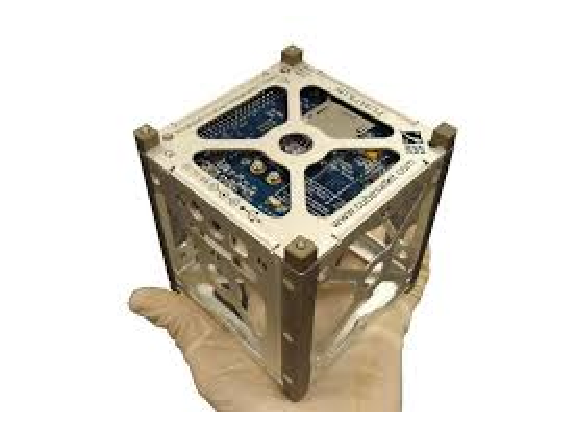
\includegraphics[width=1\linewidth]{cubesat_2}} a) \\
\caption{An example of 1U CubeSat}
\label{fig:cubesat}
\end{figure}
\end{minipage}
\hfill
\begin{minipage}[h]{0.5\linewidth}
A CubeSat (CS) is a type of miniaturized satellite for space research, these nanosatellites typically weigh between 1 and 10 kilograms and follow the popular 'CubeSat' standard,
which defines the outer dimensions of the satellite within multiple cubic units of 10x10x10 cm.
\end{minipage}
\vspace{1cm}


Utilization of a simplified infrastructure enables a low-cost platform to test the space readiness of new hardware without an exorbitant amount of prohibitive design, thus
CSs can help test new instruments or materials and validate their readiness to be integrated into a more complex space mission.
% It's pretty easy to organise satellites constellation.
The modularity of the CS allows to replace the damaged equipment thereby increasing the duration of the mission.
Moreover, the changing the configuration of the modules or adding new ones lead to changing physical characteristics of the system,
such as increasing FOV by adding extra-telescope or new wavelength band X-ray/UV/IR, all of these manipulations becomes available right in space.
It becomes really easy to organise satellites constellations to enhancing sky coverage.
In addition, there is no need thinking about space debris: cubesats burn up in the atmosphere upon re-entry.

One of the areas where CubeSats offer promise is a new type of GRB space observation instrument that is capable to pick up Gamma Ray Bursts (GRBs) in the hard X-ray to gamma band.
GRBs are broadband immense power electromagnetic flashes in space, releases energy, which is typically around $10^{44}$ J.
Observations of GRBs [6,7] play a significant role in understanding these recent discoveries [5,8].
Despite progress in investigations of GRB has been made, especially in the last decade, which culminated in the Fermi and SWIFT missions, up to the moment, some important parameters of GRB, like their prompt emission, still have not been studied well enough. 
The first direct detections of GWs [1] has brought astronomy into a new era of discovery.
The recent coincident detection of a short GRB (by Fermi and other multiwavelength partners) and a Gravitational Wave (GW) trigger has provided concrete proof that at least some short GRBs are produced by binary neutron star mergers [2,3,4,5]. The search for electromagnetic counterparts to GW sources is now more important than ever before.
CS are very useful to detect astrophysical counterparts to GW signals as well as other gamma-ray transients,
since there are oportunity to enhancing sky coverage for gamma-ray transients that is especially important since GW events can happen anywhere and anytime.

One such project is called BurstCube [11], which will provide localizations which will assist wide-field follow-up observers in afterglow detection and redshift measurement.
BurstCube will detect GRBs (long and short) from the entire unocculted sky providing broadband spectra for bursts detected elsewhere, rough localizations for follow-up, and accurately timed light curves.

This thesis is aimed at the development of a common sensor
that with a modest design adjustment can meet the needs of both landing and proximity operation Rendezvous and docking applications and also terrain mapping and navigation for a planetary exploration rover.


% There are a lot of other applications such as: Detection and rendezvous between spacecrafts and asteroids \& asteroid sample return and redirect missions; Space debris removal

% \item Optical metrology for spacecraft formation flying
% \item Examination of spacecrafts external surfaces for integrity verification and damage detection, monitoring of large de/ployable surfaces like antennas, solar panels or airbags
% \item Morphological characterization of asteroids
% \end{itemize}

% CubeSats are even being used for interplanetary missions: NASA's Mars Cube One (MarCO) will embark on a mission to Mars in May 2018. 

% A_12
% Current optical systems operate at much shorter distances, range towards the target, but they can be easily improved later.

%% more deeply about docking %%
\section{Autonomous Rendezvous And Docking}
% A_12
\begin{minipage}[H]{0.45\linewidth}
\begin{figure}[H]
\center{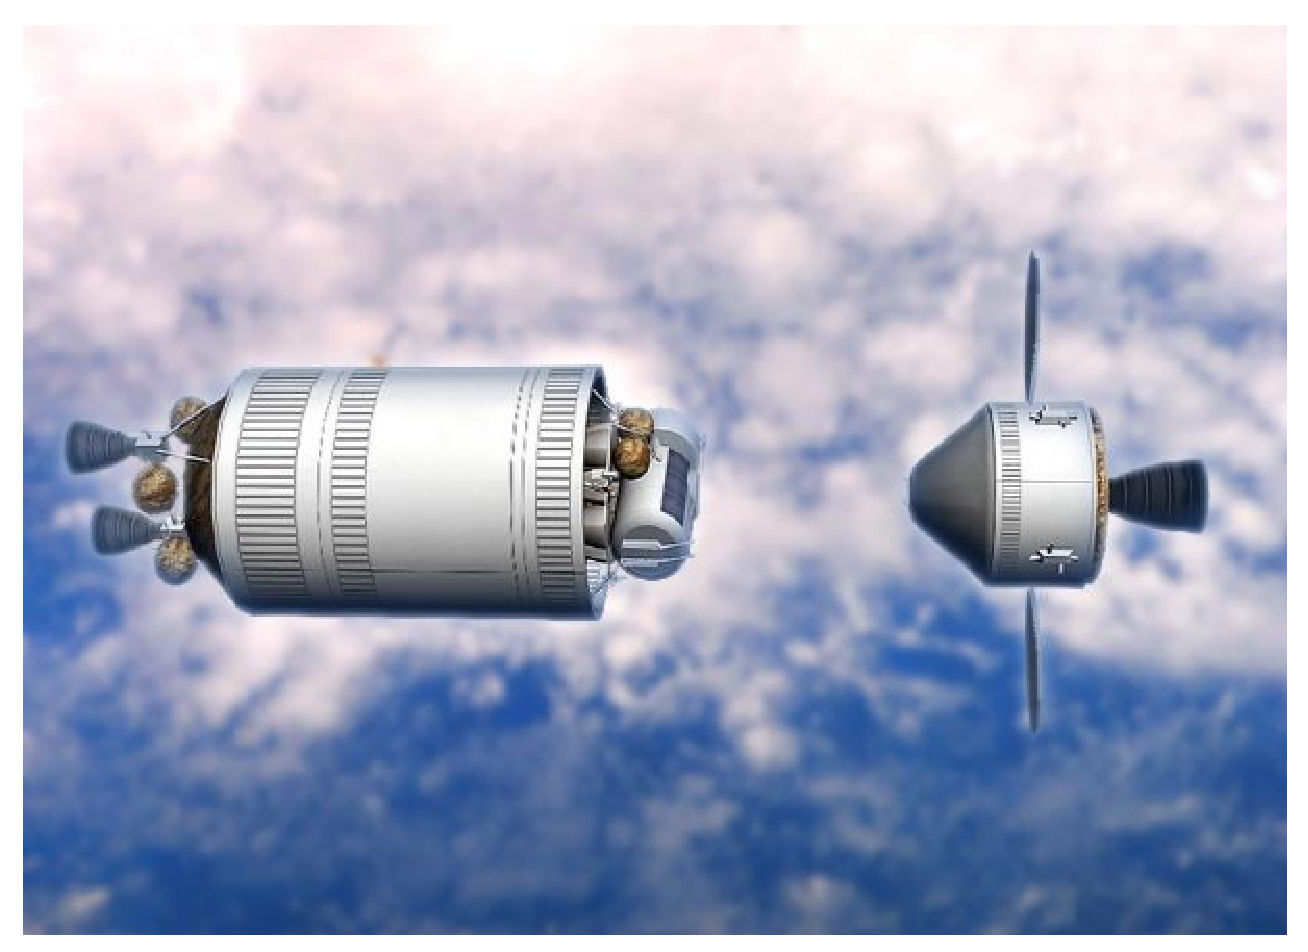
\includegraphics[width=1\linewidth]{docking}}
\caption{Orion vehicle docking with an Earth Departure Stage }
\label{fig:docking}
\end{figure}
\end{minipage}
\hfill
\begin{minipage}[h]{0.48\linewidth}
There are also number of space operations that require the ability to rendezvous and dock by an unmanned spacecraft including:
servicing satellites on-orbit; assembly of large space structures in Earth orbit; and transfer of Martian soil samples from a lander to a return spacecraft on the Mars orbit, as part of a sample return mission and even space debris removal.
\end{minipage}
\vspace{1cm}

Novel imaging sensors and computer vision technologies are required to detect a target spacecraft at a distance of several kilometers in an arbitrary orientation and to guide the approaching spacecraft to contact with the docking port. 
The ability to rendezvous and dock with no or minimum human input is considered as an integrated part of CEV (crew exploration vehicle),
which is a collection of human and robotic space systems that will allow astronauts to travel safely and cost-effectively to the Moon and Mars.
Also  this will enable the execution of fuel efficient approach trajectories and reliable operations under any illumination conditions,
as well as enabling inspection during fly around and safe station-keeping.

One of the technology that can be used for these purposes is LiDAR: detection and distance measuring method that utilizes pulsed light for measuring the distance towards an object (similar to Radar, but using light instead of radio waves).
LIDAR based sensors have gained popularity over RADAR based sensors because of their superior resolution, they also
have the advantage of long detection distance and immunity to ambient light over stereo-camera based systems.

Two optical technologies currently used for space rendezvous and docking are cameras and scanning laser rangefinders.
The camera based systems typically operate at ranges of up to 100m and the maximum range is limited by a trade-off between
the camera image resolution (which is drastically decreasing like square of distance) and field of view, and the size and separation of visual targets.
Scanning laser rangefinders use beam steering devices to direct a laser beam to objects in the scene and rely on either a triangulation principle,
a measure the phase shift (continuous wave), but the most mature and widely used LIDAR technology in space operation is pulse laser based TOF (time-of-flight) LIDAR,
which measure time between sending and returning of the signal.
Emergence of novel LIDAR technologies and computer vision algorithms will lead to a new generation of rendezvous and docking systems in the near future.
Such systems will be capable of autonomously detecting a target satellite at a distance of a few kilometers, estimating its bearing, range and relative orientation under virtually any illumination, and in any satellite pose.

The data from the scanning rangefinder must be processed by a vision system to compute the information, such as
distance, bearing, pose, that is required by the Guidance, Navigation and Control unit of the autonomous service
spacecraft. Some easy to reproduce, semi-analytic calibration approach [A7] is developed
for hardware-in-the-loop performance assessment of pose determination algorithms processing point
cloud data, collected by imaging a non-cooperative target with LIDARs. 


Although laser ranging and scanning sensors are widely used in a variety of industries, a sensor designed for spacecraft
operations, including autonomous rendezvous, inspection and servicing remains a challenge. This is primarily due to
critical requirements, including the need to have simultaneous high sampling speed, and good range and lateral
resolution at both short range of a few meters and at long range of a few hundred meters.

\subsection{Review of existing system}

Up to the present moment, all LiDAR systems used in space are heavy, bulky and have big power
consumption, which makes it impossible to use them on the CubeSats. 
LIDARs flown on Previous Spacecraft:
ASC’s DragonEye,  Ball’s Vision Navigation Sensor (VNS), RendezVous Sensor (RVS) / Telegoniometer (TGM) on HTV / ATV, Videometer (VDM) on the ESA Automated Transfer Vehicle (ATV), Trajectory Control Sensor (TCS) on the Space Shuttle. All of them passed the test of time, but replace them came new technologies.

\subsubsection{The Jena-Optronik RVS Rendezvous and Docking Sensor}
The Jena-Optronik RVS Rendezvous and Docking Sensor is the most frequently used LIDAR
sensor for docking to the International Space Station ISS.
RVS3000  is the advanced 3D imaging LIDAR for rendezvous and docking (Fig.~\ref{fig:jena}).
Acquisition, tracking and imaging of both cooperative and non-cooperative targets.

\begin{figure}[H]
\begin{floatrow}
\ffigbox{
\center{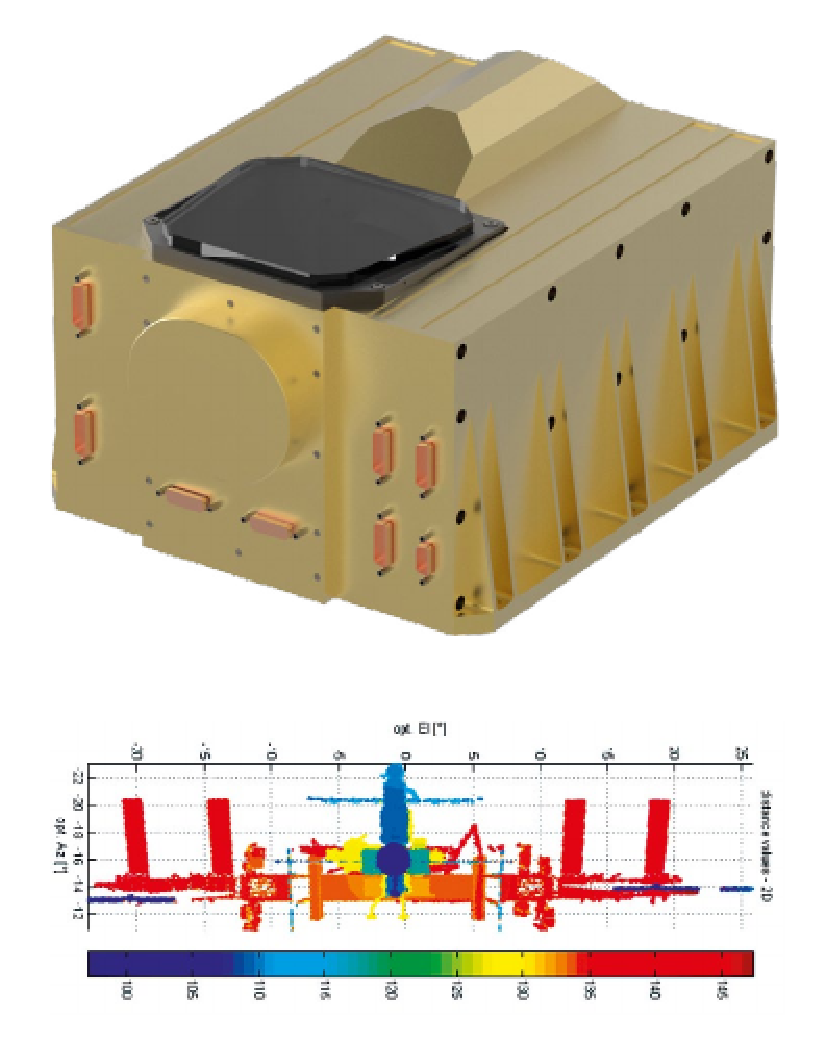
\includegraphics[width=0.8\linewidth]{jena}} 
}{
  \caption{Upper side is RVS3000. \\Bottom one is ISS snapshoted by RVS3000.}%
\label{fig:jena} % or change caption location
}
\capbtabbox{
\begin{tabular}{|M{3cm}|M{3cm}|}
\hline
Field-of-View: & \textbf{40$\pmb{{^\circ}}$ x 40$\pmb{{^\circ}}$}  \\ \hline
Wavelength: & \textbf{910 nm} \\  \hline
Operating range against cooperative targets: & \textbf{< 1500 m} \\  \hline
Operating range against non-cooperative targets: & \textbf{< 250 m} \\  \hline
Image frame rate: & \textbf{up to 2 Hz} \\  \hline
Power consumption: & \textbf{40 W} \\  \hline
Dimension: & \textbf{575 x 569 x 371 mm} \\  \hline
Mass: & \textbf{14.5 kg} \\  \hline
\end{tabular}
}{%
\caption{RVS3000 characteristics}
\label{tbl:jena_characteristics}
}
\end{floatrow}
\end{figure}

Despite the fact that they are leaders in RVS systems, the Lidar has the parameters presented in Table ~\ref{tbl:jena_characteristics}.
Which making this RVS absolutely not applicable for using at small satellites.

\subsubsection{LIRIS}
Another new set of optical sensors for non-cooperative rendezvous and docking, called “LIRIS” (Laser Infra-Red Imaging Sensors) desribed more detailed in [A9]
As part of this project, a prototype for a new 3D Imaging LIDAR was developed, integrated and tested. Fig. \ref{fig:LIRIS}
\begin{figure}[h]
\begin{floatrow}
\ffigbox{
\center{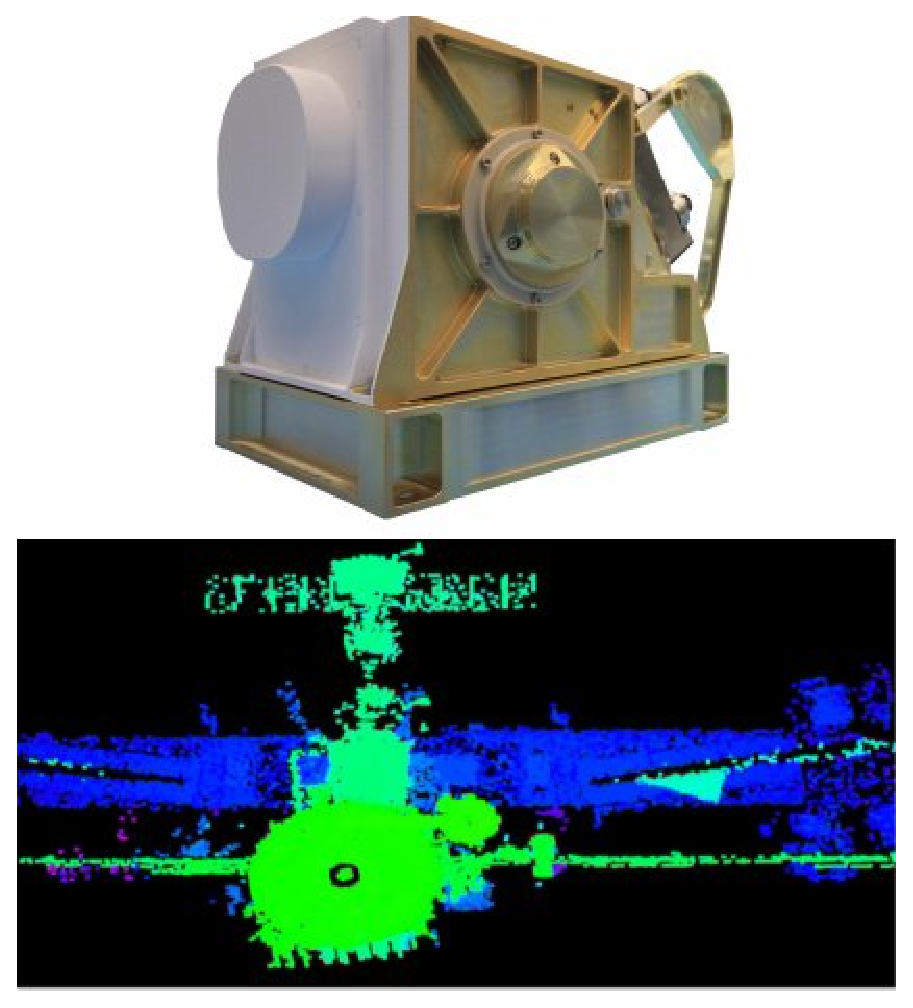
\includegraphics[width=0.8\linewidth]{liris}} 
}{
  \caption{Upper side is LIRIS. \\Bottom one is ISS snapshoted by LIRIS.}%
\label{fig:LIRIS} % or change caption location
}
\capbtabbox{
\begin{tabular}{|M{3cm}|M{2.5cm}|}
\hline
Field-of-View: & \textbf{40$\pmb{{^\circ}}$ x 40$\pmb{{^\circ}}$}  \\ \hline
Wavelength: & \textbf{1550 nm} \\  \hline
Operating range against cooperative targets: & \textbf{< 3500 m} \\  \hline
Operating range against non-cooperative targets: & \textbf{< 260 m} \\  \hline
Image frame rate: & \textbf{up to 3 Hz} \\  \hline
Power consumption: & \textbf{35 W} \\  \hline
Dimension: & \textbf{292 x 465 x 385 mm} \\  \hline
Mass: & \textbf{13.1 kg} \\  \hline
\end{tabular}
}{%
\caption{LIRIS characteristics}
\label{tbl:liris_datasheet}
}
\end{floatrow}
\end{figure}

Same here, dimesion and size (Table \ref{tbl:liris_datasheet}) making this RVS absolutely not applicable for using at small satellites.


\subsubsection{Neptec's TriDAR}
\begin{minipage}[h]{0.40\linewidth}
\begin{figure}[H]
\center{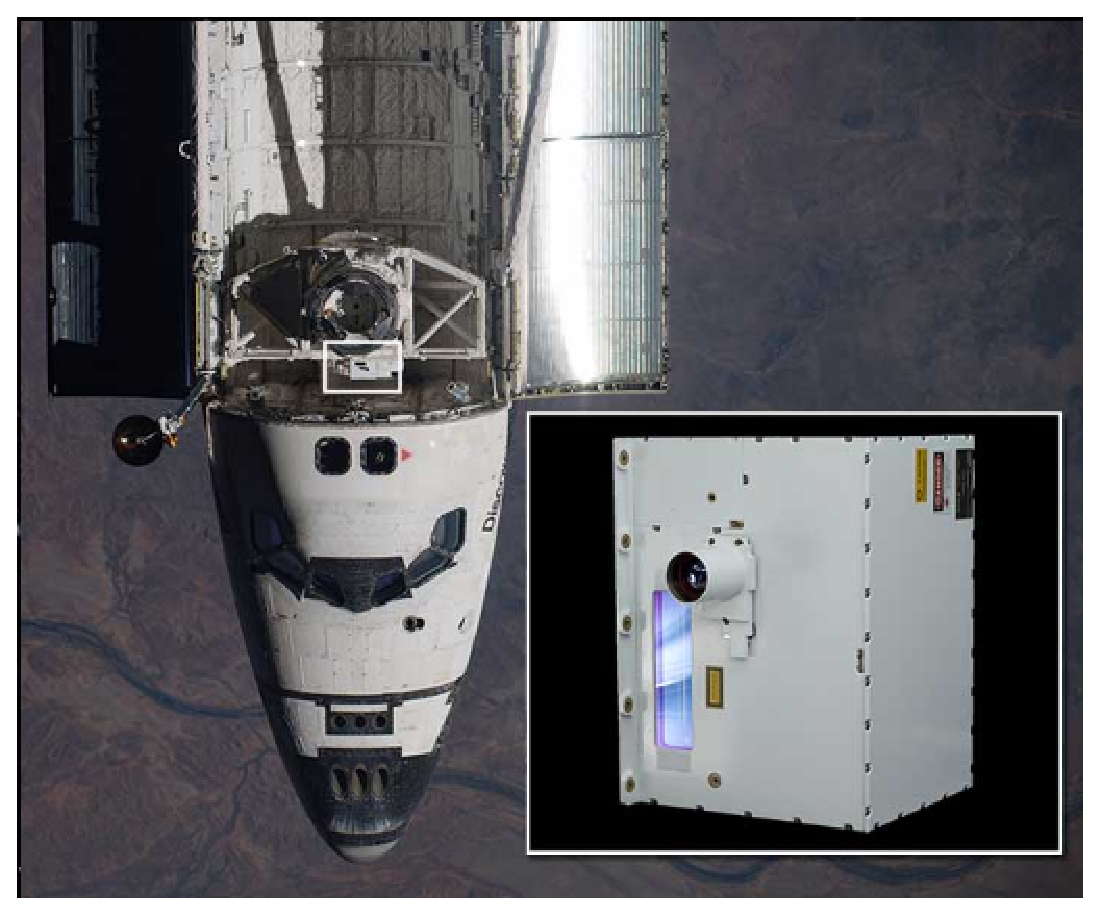
\includegraphics[width=1\linewidth]{tridar}} a) \\
\caption{Neptec's TriDAR module}
\label{fig:cubesat}
\end{figure}
\end{minipage}
\hfill
\begin{minipage}[h]{0.48\linewidth}
Neptec’s TriDAR was specifically designed for non-cooperative missions such as satellite servicing which require high levels of autonomy.
This allows the sensor to be adapted to rendezvous and dock to different targets and approach profiles even after launch.
% It now serves as a primary rendezvous and docking sensor for the Cygnus spacecraft for cargo resupply missions to the International Space Station (ISS).
Unfortunately, there is no free access to the information about the parameters of the system, but one can say with confidence that they do not exceed RVS3000 / LIRIS, since TriDAR was released much earlier.
\end{minipage}
\vspace{1cm}
\subsection{Spacecraft Landing Applications}
Lidar can be recognized as a primary candidate sensor for safe precision landing on solar system bodies (Moon, Mars, Jupiter and Saturn moons, etc.).
For future robotic missions to the Moon and Mars that require
landing at pre-designated sites of high scientific value, while avoiding hazardous terrain features, such as escarpments, craters, slopes, and rocks.
During the final stages of landing (Approach Phase at fig ~\ref{fig:landing}), from about 1 km to 500 m above the ground, the 
lidar can generate 3-dimensional images of the terrain to identify hazardous features such as craters, rocks, and steep slopes. The onboard flight computer then can use the 3-D map of terrain to guide the vehicle to a safe location.

\begin{figure}[h]
\center{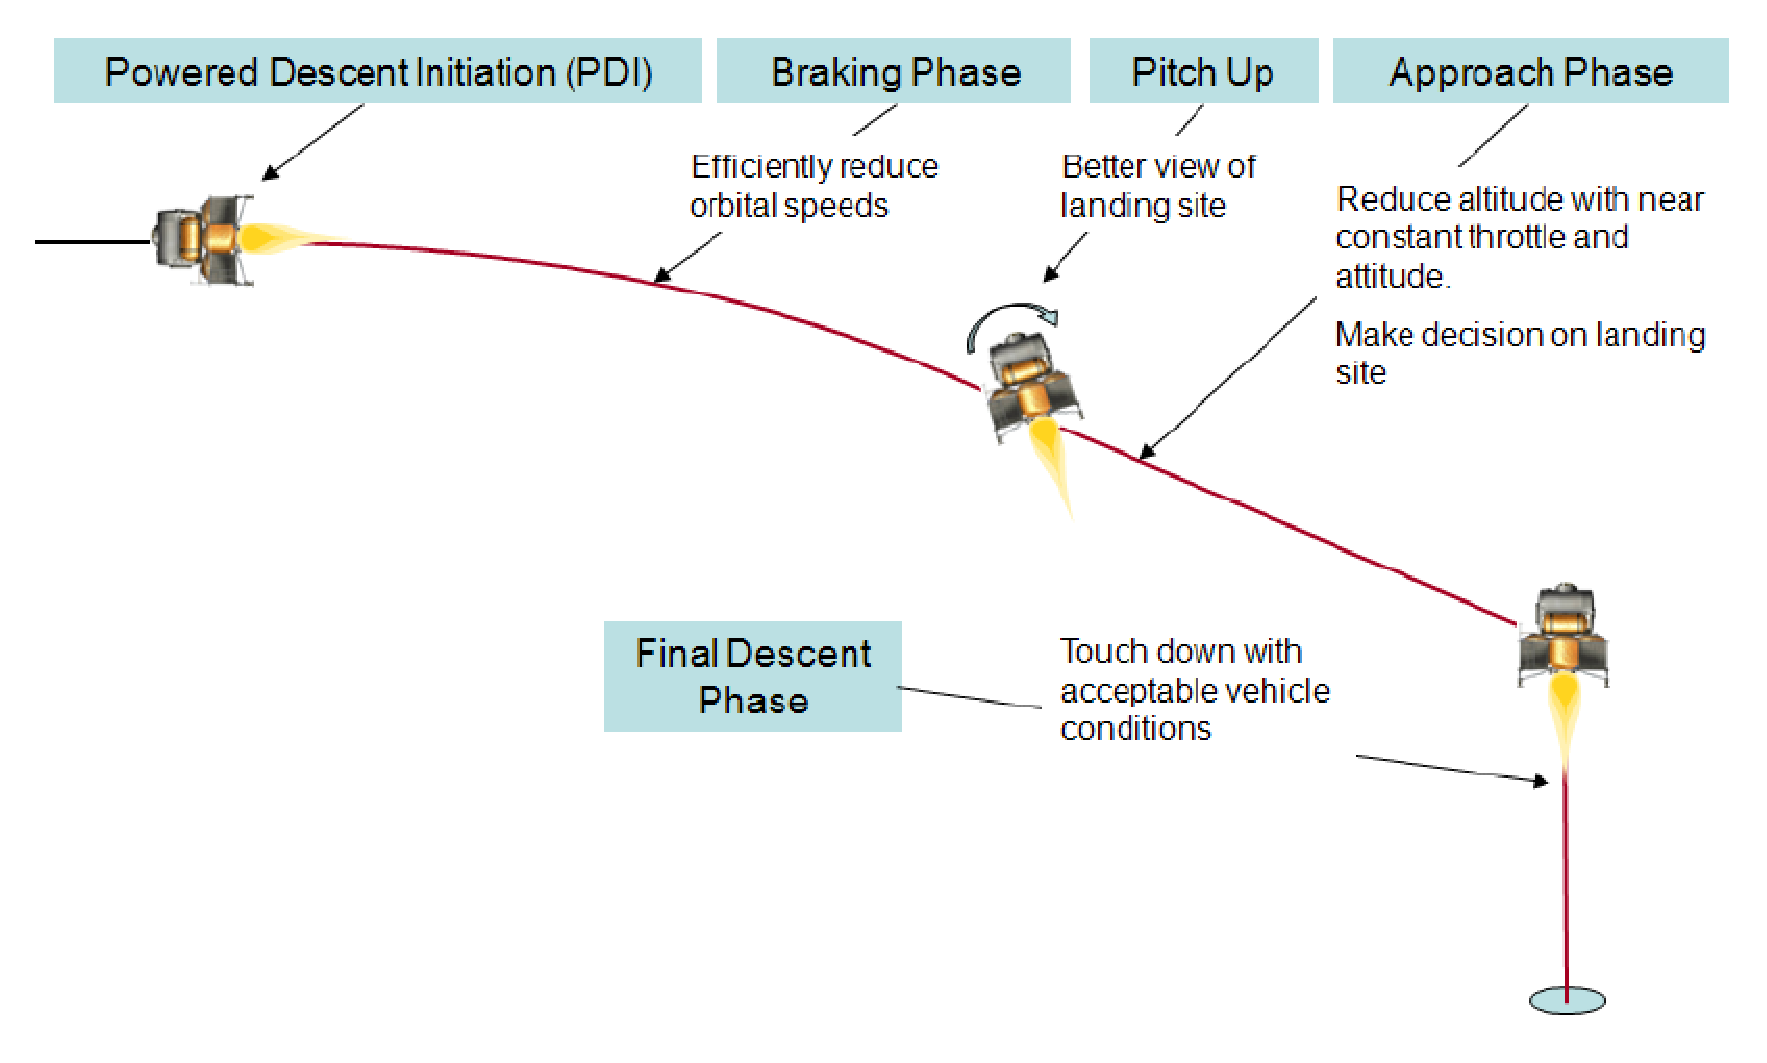
\includegraphics[height=9cm, width=1\linewidth]{land}} 
  \caption{Typical Lunar descent and landing phase}%
\label{fig:landing} % or change caption location
\end{figure}

According to [A8, A2], the minimum requirements which should be satisfied in lidar system are represented in Table \ref{tbl:landing_datasheet}:



\begin{figure}[h]
\begin{floatrow}
\ffigbox{
\center{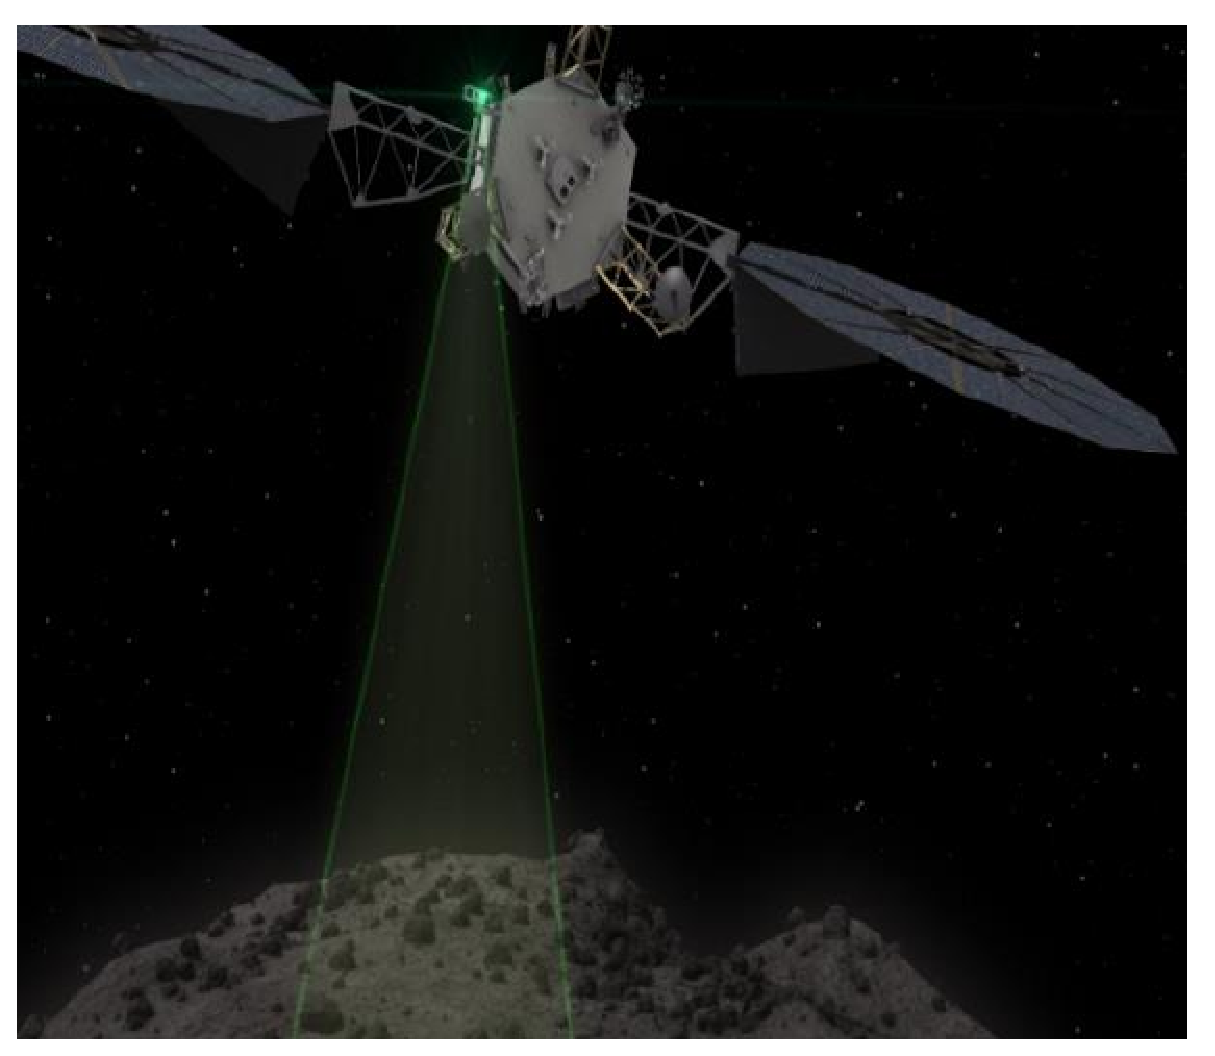
\includegraphics[height=4cm, width=1\linewidth]{asteroid_grab}} 
}{
  \caption{Lidar sensor characterizing an asteroid surface before terminal approach for collecting samples or capturing a boulder}%
\label{fig:asteroid_grab} % or change caption location
}
\capbtabbox{

\begin{tabular}{|M{2.5cm}|M{2.5cm}|}
\hline
Range: & \textbf{0 to 5000 m}  \\ \hline
Field of View: & \textbf{> 20$\pmb{{^\circ}}$ x 20$\pmb{{^\circ}}$} \\  \hline
Spatial Resolution: & \textbf{<0.25m at 300m} \\  \hline
Range accuracy: & \textbf{<5m(5km) <0.1m (300m)
<0.02m (10m)} \\  \hline
Image frame rate: & \textbf{> 1Hz} \\  \hline
\end{tabular}
}{%
\caption{The minimum requirements which should be satisfied in lidar system for landing}
\label{tbl:landing_datasheet}
}
\end{floatrow}
\end{figure}


One more application comes from studying of morphological characterization of asteroids, the lidar can analyze asteroid surface before terminal approach (Fig. ~\ref{fig:asteroid_grab}).


\subsubsection{Our solution for Rendezvous And Docking}
Advance of sensor technologies and novel tracking algorithms has led to a few new approaches of autonomous rendezvous and dock,
but it still typically requires multiple systems to complete the operation. It is desirable to have one system that can do the tracking at all distances. 
Reducing the number of sensors necessary to cover the required range of distances (preferably to one) has significant
benefits due the reduced launch mass and volume, and lower power requirements.

At our Labaratory we have developed such vision system based on a scanning LIDAR to get real-time 3D picture.
Our LiDAR consumes much less power (~5W) and has an incredible small mass (<500g) and size of a matchbox, while is able to track satellite pose with high accuracy and high frame rate.





\section{Terrain Mapping and Navigation for a Planetary Exploration Rover
}

%% 1041
In recent decades, terrain modelling and reconstruction techniques have increased research
interest in precise short and long distance autonomous navigation, localisation and mapping within field robotics. One of the most challenging applications is in relation to autonomous planetary exploration using mobile robots.
Rover navigation on planetary surfaces can be extremely hazardous, which includes vehicle rollover on sloped terrain, or immobilizing wheel slippage on loose sand. That is why high
resolution topographic data is required to ensure rover safety and mission success. 
A terrain feature information can be exploited to assess
obstacle size, slope angle, or terrain roughness so that
the rover is able to find its heading for travel.

The farther an explored planet is, the longer it would take a commanding signal to reach from an earth commanding station to planet exploring rover.
Thus, it is necessary for a space rover to be capable of autonomous and semi-autonomous decision making such as localization, navigation, and environmental mapping, with little intervention from ground control at very high traverse speeds. Missions that require absolute rover localisation remain a challenging problem due to the absence of helping technologies such as Global Positioning Systems (GPS) on extraterrestrial planets.

The majority of the rover onboard vision systems in past and current missions (such as, Mars
Exploration Rover (MER), Mars Science Laboratory (MSL) and Exobiology on Mars (ExoMars)) use
cameras for terrain perception, such as; stereopsis for autonomous rover navigation (e.g., visual odometry), hazard detection (e.g., slip perception) and scientific study (e.g., MSL ChemCam) [5] % sensors

The drawbacks of the camera-based terrain mapping are that
a stereo matching process is generally a time-consuming task(finding correlation between 2 frames of cameras) for the low-power flight CPU of the rover, requiring relatively long computational time, especially higher resolution cameras are used. [3]. Additionally, the
quality of visual information may vary with the intensity of sunlight/shadows. %% ISAIRA_2012 (A5)
Also, there is a significant decrease in the accuracy of the estimated depth Z with the increase in distance from the camera (Eq. \ref{eq:stereo_error}), which may not be deemed suitable for long range terrain modelling and perception. 



\begin{figure}[H]
\begin{minipage}[h]{0.4\linewidth}
\center{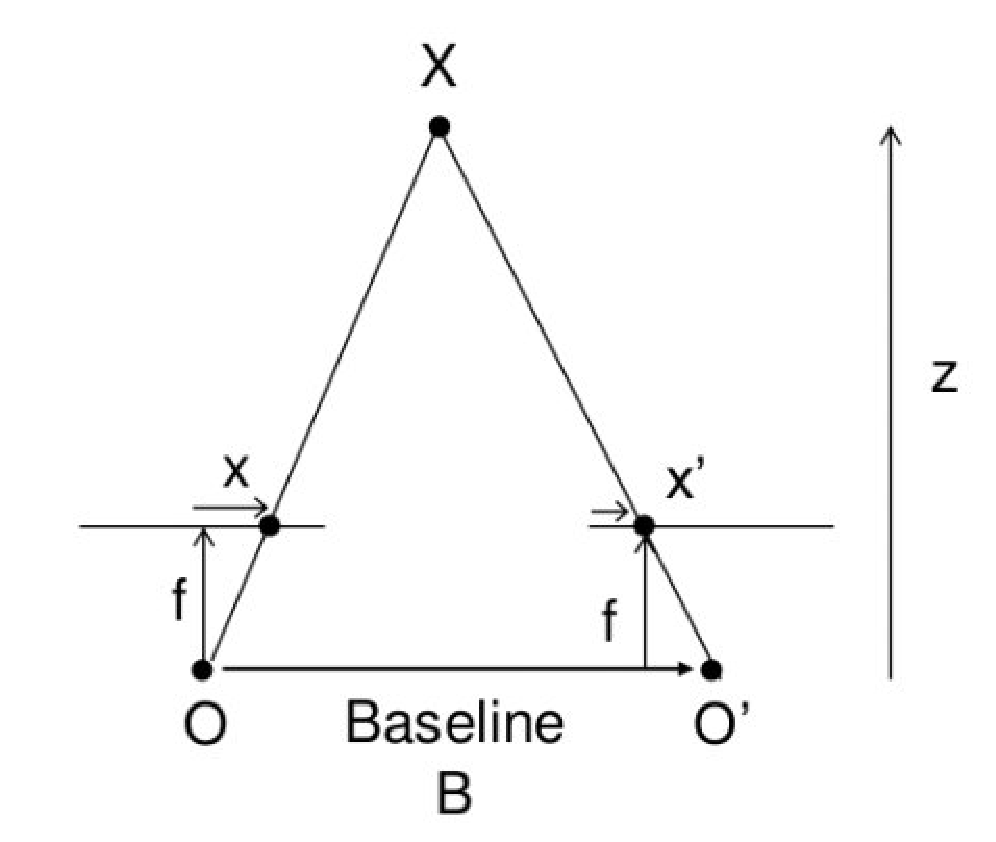
\includegraphics[width=1.2\linewidth]{stereo}}
\end{minipage}
\hfill
\begin{minipage}[h]{0.45\linewidth}

The left diagram contains equivalent triangles. Writing their equivalent equations will yield us following result:

\begin{equation}\label{eq:stereo_eq}
z=f \cdot \frac{B}{d}
\end{equation}

Where f is focal length, B is baseline, $d = x-x'$. Here d is known as the disparity.

\end{minipage}
\caption{
A simple stereo geometry
}
\label{fig:lens}
\end{figure}




From Eq \ref{eq:stereo_eq} by differentiating, for depth error we got:

\begin{equation}\label{eq:stereo_error}
\delta z =  \frac{z^2}{f \cdot B} \cdot \delta d
\end{equation}

As can be seen from Eq. \ref{eq:stereo_error} depth resolution is proportional to the square of the depth (Z) and is inversely proportional to the focal length (f) and baseline (B), or distance between the cameras.
Good depth resolution requires a large baseline (B) value, a large focal length (f) value and a small depth (Z) value.
Depth resolution depends on accurate disparity estimations. The accuracy of disparity estimation is directly proportional to pixel size, where smaller pixel sizes provide better resolution. Typically, disparity can be estimated accurately to about one fifth of a pixel. For a camera with a pixel size of 7.5 microns, this translates to a disparity resolution of 1.5 microns. 

Hence stereopsis does not provide an optimal solution beyond a few metres from the rover for future more challenging planetary rover missions.

Another technique for the terrain mapping involves the use of a lidar that can determine a distance from a laser emitter to an object based on the time of flight principle,
this technology been used extensively for precise long and short target detection, identification, and depth estimation.
Extensive research and development for using the LIDAR technique in
a terrain feature mapping and terrain classification described in [5]–[8].
Comparing the LIDAR-based terrain mapping to the camera-based one, the LIDAR can directly measure
three-dimensional distances from the sensor to the objects, providing “point cloud” data of the scene without any additional processes (the camera-based mapping needs stereo matching for the 3D mapping). 
After that, the point cloud data of the terrain features provided by the LIDAR are converted into a digital elevation map with
a sector-shaped reference grid  for the DEM conversion, termed as $C^2DEM$.


\begin{minipage}[h]{0.45\linewidth}
\begin{figure}[H]
\center{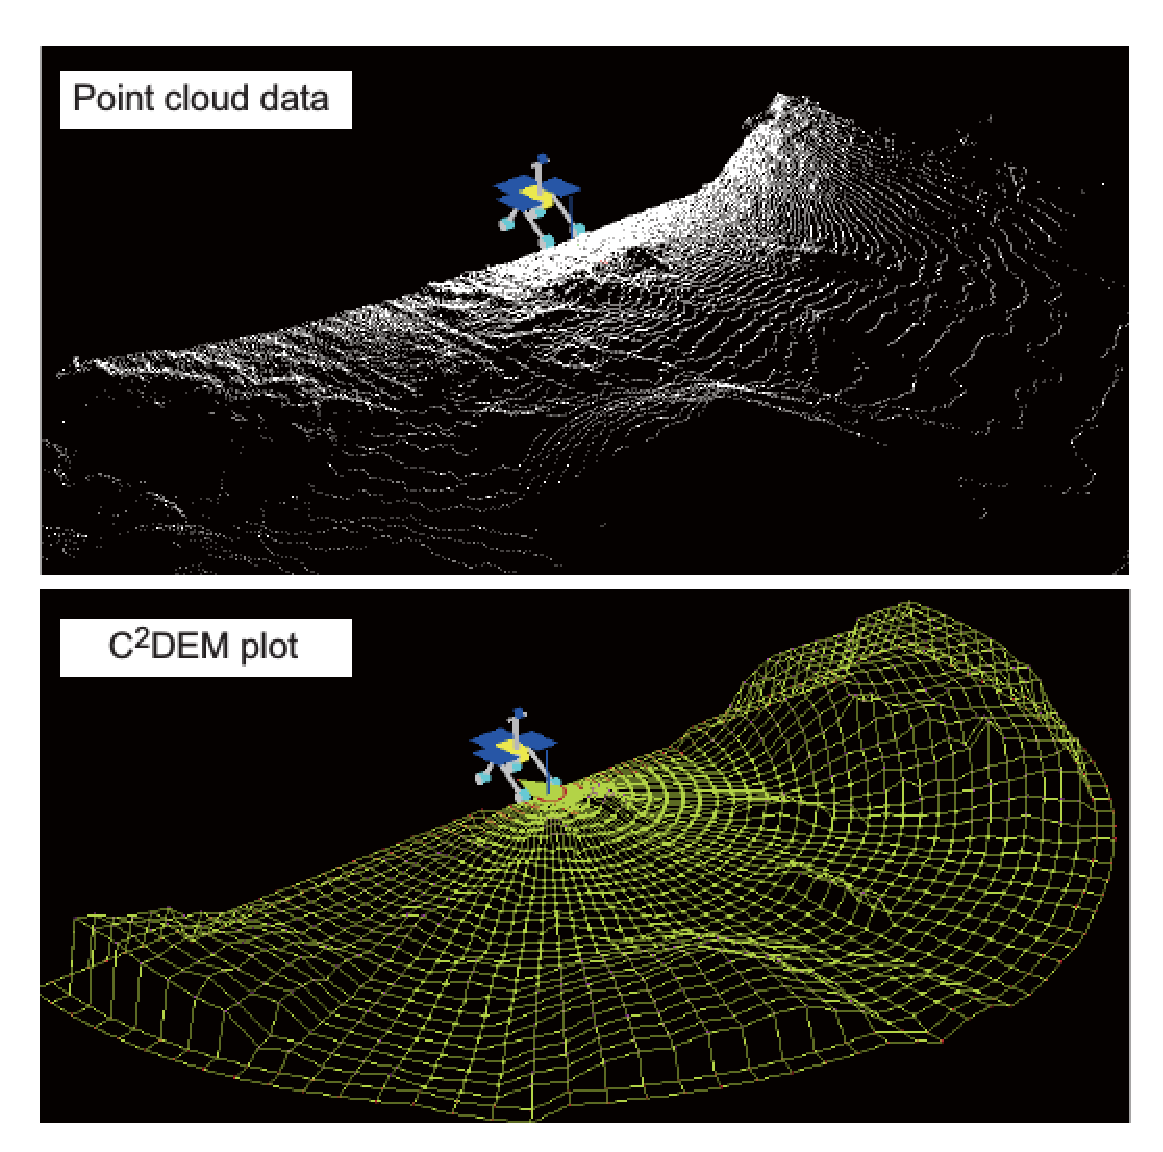
\includegraphics[width=1\linewidth]{DEC}} 
\caption{An example of point cloud to $C^2DEM$ transformation.}
\label{fig:DEC}
\end{figure}
\end{minipage}
\hfill
\begin{minipage}[h]{0.48\linewidth}
An example of $C^2DEM$ conversion from a point cloud data is shown in Fig. \ref{fig:DEC}.
The terrain mapping with the $C^2DEM$ achieves detailed representation of the terrain near the rover as well as wide selectivity of the rover look-ahead directions.
Finally, the path planning algorithm considering three indices: terrain inclination, terrain roughness, and path length makes decision about  the path.

\end{minipage}
\vspace{1cm}

Lidar-based terrain mapping and navigation for a planetary exploration rover was succesfully tested in [ISA2012] by using motorable lidar made by Hokuyo. Vision system of this rover uses both stereo-cameras and lidar placed at 2-axis rotatable fimbale (Fig.\ref{fig:rover}).



\begin{figure}[H]
\begin{floatrow}
\ffigbox{
\center{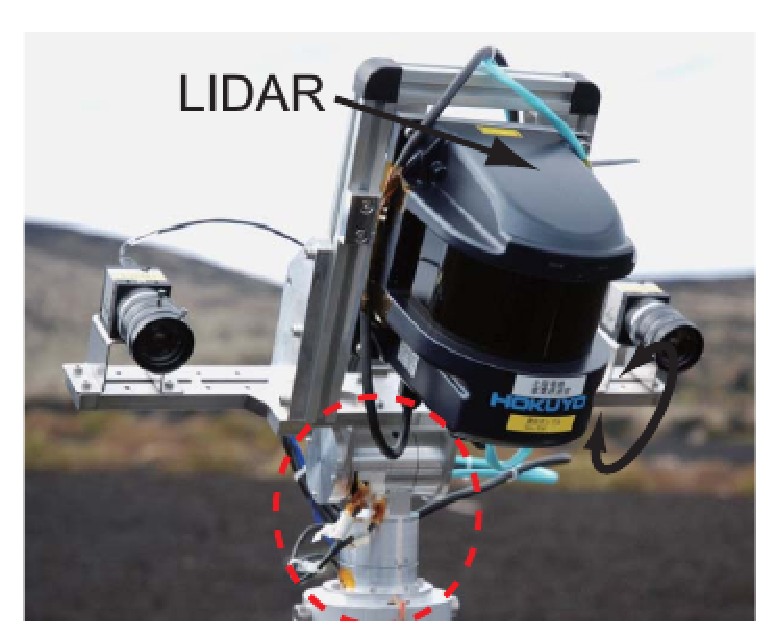
\includegraphics[width=1\linewidth]{rover}} 
}{
	\vspace{-0.5cm}
  \caption{Gimbaled-LIDAR system for terrain mapping.}%
\label{fig:rover} % or change caption location
}

\capbtabbox{

\begin{tabular}{|M{2.5cm}|M{3.5cm}|}
\hline
Scanning range: & \textbf{0.1 to 30m} \\  \hline
Wavelength: & \textbf{905 nm} \\  \hline
Field of View: & \textbf{20$\pmb{{^\circ}}$ x 190$\pmb{{^\circ}}$} \\  \hline
Scanning angle resolution: & \textbf{0.25$\pmb{{^\circ}}$} \\  \hline
Range accuracy: & \textbf{$\pm$ 0.1 m} \\  \hline
Image frame rate: & \textbf{> 1Hz} \\  \hline
Power consumption: & \textbf{6 W} \\  \hline
Dimensions: & \textbf{124 x 126 x 150mm} \\  \hline
Weight: & \textbf{800 g} \\  \hline

\end{tabular}
}{%
\caption{Specification of the LIDAR scanning system}
\label{tbl:landing_datasheet}
}

\end{floatrow}
\end{figure}




Clearly that LiDAR has a key-role in rover navigation, it covers both short range and long range.
Additionally to be easy-to use and therefore adapted to fast-making decisions, like multi-path planning that is used for an
autonomous mobility of a planetary exploration rover.
The data allows cm-precise estimations of distances, heights and slopes, which are critical for safe rover displacement as well as remote and contact science operations.
It also allows extremely detailed surface mapping of objects and therefore has implications for our knowledge of planetary surfaces.
A drawback of the LIDAR-based mapping is that the LIDAR cannot obtain pure color data of the terrain (in
grayscale or RGB) even though it can measure the distance as well as intensity of the light reflected from objects.
Therefore, a possible future realization will be forwarded to enables three-dimensional mapping with color of the terrain.

\subsection{Our solution for Korean Lunar Exploration Program}
Our laboratory developed a LiDAR submodule with the size of a matchbox. This LiDAR
consumes little power and has a small mass. The LiDAR submodule (or a set of several submodules)
is suitable for close distance scanning, and it is perfect for Mars and Lunar rovers because it can
allow them to make detailed scans of the surrounding without considerable payload losses. The
concept we are developing (MEMS pinhole), basically, is a unique technology that allows not only
LiDARs development, but also other scientific instruments, such as spectrometers or cameras.
Thus, our lidar can be easily integrated for the Korean Lunar Exploration Program for use in a lunar rover.

% Being incredibly small and light, while consuming little power, and having good performance our lidar

%% OUR LIDAR concept/solution%%%

\section{About ISS-gamma mission(can be checked in space)}
Preflight test can be done in ISS gamma exp (we can detect trash to check wheter it working or not).

% The aim of thise thesis is making lidar which can be used like rendevouz \& rover.

\section{Outline}
This thesis is organized as follows. In chapter 2, I describe 
% my preflight work on the SMT,
% which consists of updates of the onboard FPGA firmware and the reasons for them. In chapter 3, I
% explain the problems that occurred with the SMT hardware in space and the means of its recovery,
% which was found with a preflight model of the UFFO (PFM). Then, in chapter 4, I report on the
% results of the SMT imaging and motor performance tests. Chapter 5 provides an overview of the
% observations made by the SMT in space. Finally, I present a summary in chapter 6.
